\documentclass[border=5mm]{standalone}
\usepackage{tikz}
\usepackage{amsmath,amssymb}
\usetikzlibrary{positioning,arrows.meta}

\begin{document}
% Narrow responsive map: inputs flow down to a shared representation, which
% branches into parameter-specific heads and their outputs.
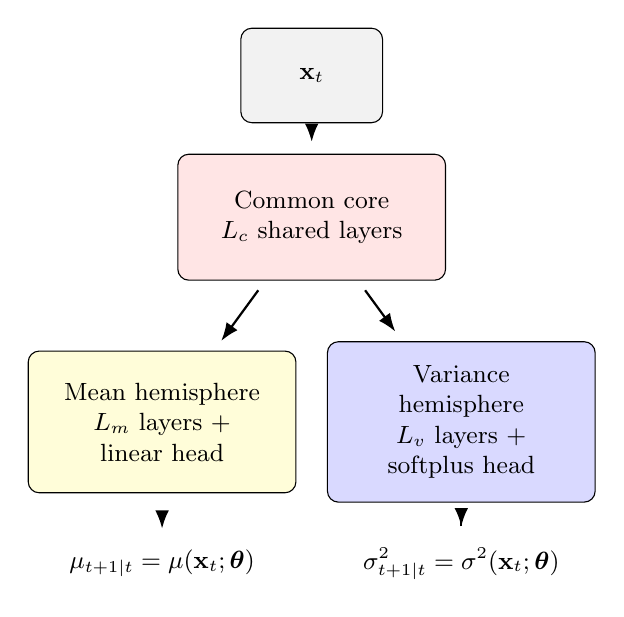
\begin{tikzpicture}[
  font=\small,
  inputblock/.style={draw, rounded corners, fill=gray!10, align=center,
    minimum width=1.8cm, minimum height=1.2cm, text width=1.0cm, inner sep=3mm},
  coreblock/.style={draw, rounded corners, fill=red!10, align=center,
    minimum width=3.4cm, minimum height=1.6cm, text width=2.7cm, inner sep=3mm},
  meanblock/.style={draw, rounded corners, fill=yellow!15, align=center,
    minimum width=3.4cm, minimum height=1.8cm, text width=2.7cm, inner sep=3mm},
  varblock/.style={draw, rounded corners, fill=blue!15, align=center,
    minimum width=3.4cm, minimum height=1.8cm, text width=2.7cm, inner sep=3mm},
  flow/.style={thick,-{Latex},shorten >=1.5mm,shorten <=1.5mm},
  outputflow/.style={thick,-{Latex},shorten >=1.5mm,shorten <=3mm}
]
\node[inputblock] (x) at (0,6.0) {$\mathbf{x}_t$};
\node[coreblock] (core1) at (0,4.2) {Common core\\$L_c$ shared layers};
\node[meanblock] (mean) at (-1.9,1.6)
  {Mean hemisphere\\$L_m$ layers + linear head};
\node[varblock] (var) at (1.9,1.6)
  {Variance hemisphere\\$L_v$ layers + softplus head};
% Two-index labels are wider: at \small each is about 3.3 cm, so with centers
% 3.8 cm apart the gap is about 0.5 cm. Positivity of the variance is stated in
% the caption and by the softplus head, so the label omits "> 0".
\node (mu) at (-1.9,-0.2)
  {$\mu_{t+1\mid t}=\mu(\mathbf{x}_t;\boldsymbol{\theta})$};
\node (sig2) at (1.9,-0.2)
  {$\sigma_{t+1\mid t}^2=\sigma^2(\mathbf{x}_t;\boldsymbol{\theta})$};
\draw[flow] (x) -- (core1);
\draw[flow] (core1) -- (mean);
\draw[flow] (core1) -- (var);
\draw[outputflow] (mean) -- (mu);
\draw[outputflow] (var) -- (sig2);
\end{tikzpicture}
\end{document}
